\documentclass[sigconf]{acmart}
\sloppy
\usepackage{graphicx}
\settopmatter{printacmref=false} % Removes citation information below abstract
\renewcommand\footnotetextcopyrightpermission[1]{} % removes footnote with conference information in first column
\pagestyle{plain} % removes running headers
\makeatletter
\renewcommand\@formatdoi[1]{\ignorespaces}
\makeatother
\settopmatter{printacmref=false}

\usepackage{booktabs} % For formal tables
\setcopyright{none}

\newcommand{\MITAffiliation}{
\affiliation{%
  \institution{Massachussets Institute of Technology}
  \streetaddress{32 Vassar Street}
  \city{Cambridge}
  \state{Massachussets}
  \country{USA}
  \postcode{02139}
}}
 
 \newcommand{\EPFLAffiliation}{
\affiliation{%
  \institution{Swiss Federal Institute of Technology in Lausanne (EPFL)}
  \streetaddress{Route Cantonale}
  \city{Lausanne}
  \country{Switzerland}
  \postcode{02139}
}}

\begin{document}
\title{ShrinkNets}

\author{Guillaume Leclerc}
\authornote{Visiting Student}
\MITAffiliation
\email{leclerc@mit.edu}

\author{Raul Castro Fernandez}
\MITAffiliation
\email{raulcf@csail.mit.edu}

\author{Samuel Madden}
\MITAffiliation
\email{madden@csail.mit.edu}


% The default list of authors is too long for headers.
\renewcommand{\shortauthors}{G. Leclerc et al.}


\begin{abstract}
  Write the abstract at the end !
\end{abstract}


\maketitle

\section{Introduction}

When designing Neural Netowrks, finding the apropriate size (width and depth) is key. Indeed, these hyper parameters have a strong correlation with over/underfitting. The main problem is that we have no reliable way to find them [ref]. Decades of experimentation led to some heuristics [ref] that try to prune that immense space of possible network sizes, but we are still bound to use costly and sometimes complex methods to find reasonable values for these hyper-parameters.

% \subsection{Main Contributions}
% 
% The main contribution of this article are:
% \begin{itemize}
%   \item The Filter layer, a neural network layer which puropose is to allow feature selection
%   \item To the best of our knowledge, the first attempts to dynamically change the number of channels in deep convolutional neural networks
%   \item A deep learning library built on top of PyTorch that allow partictionners to train shrinking networks (Feed-Forward and Convolutional)
% \end{itemize}
% 
\section{Related Work}

\par In the litterature we can see different ways of approaching this issue. The first one is to select parameters, train the model, evaluate it, repeat and pick the best one. There are many different ways of selecting parameters: random search [ref], grid search [ref], meta gradient descent [ref], parsen trees[ref], gaussian processes [ref] etc... but they all suffer from one major drawback: we have to train and evaluate countless models; and even if some algorithms allow parallel evaluations [ref] to reduce the overall training time, the hardware and energy cost is still important.
\par To reduce the number of models trained, another approach emerged: train a slightly bigger model and after convergence, remove as many parameters as possible without impacting the performance of the model. Notable contributions are Optimal Brain Dammage [ref], Deep Compression [ref], and Group sparsity [ref] (this one is especially related to this article). These techniques are very interesting but they still require a reasonable network size to start with, so they usually have to be combined with classic hyper-optimization techniques.
\par However, some recent contributions like Non-Parametric Neural Netowrks [ref] and [ref] try to learn the network size (width for the former and depth for the latter) during the training process and without any prior assumption about the network size.

\section{The Filter Layer}
\subsection{Motivation}

The method described in [ref] grows and shrink the network over time. Though it seems to be an attractive property to have, during our experiments and according to their results, models are very slow to train and sometimes converge to suboptimal solutions. Their method also required a new optimizer \textit{AdaRad}. Our goal was to provide a solution that can easily be integrated in existing machine learning systems and provide similar convergence speed and accuracy. Therefore, designing a new layer that only allow seemed to be best approach.

\subsection{Definition}

In this section we define the \textit{Filter Layer}. It takes an input of size $\left(B \times C \times D_1 \times \dots \times D_n\right)$. So it is compatible with fully connected layers with $n=0$ or convolutional layers with $n=2$. This layer has a parameter $\theta \in \mathbb{R}^C$ and is defined the following way.
\begin{equation}
  Filter(I;\theta) = I \circ \max(0, \theta)
\end{equation}

Where $\circ$ is the Hadamard product (pointwise multiplication), and $\theta$ is expanded in all dimensions except the second one to match the input size. It is easy to see that if for any $k$, if $\theta_k \leq 0$, the $k^{\text{th}}$ feature/channel will forever be $0$. We can use this property to devise a training procedure.
\subsection{The training procedure}

To train networks we need start with a clearly oversized network, then we insert \textit{Filter Layers} in the architecture (usually after every Linear or Convolutional layer except the last one) and we sample their weight from the $\text{Uniform}(0, 1)$ distribution. We could train this network as it is and it would be equivalent to a normal neural netork. However, our goal is to find the smallest network with reasonable performance. We can achieve that by introducing sparsity in the parameters of the \textit{Filter Layers}. Indeed, having a negative value is equivalent to zeroing an entire row and column in the surrounding layers. These disabled neurons/channels can be removed from the network without changing its output. To obtain this sparsity we simply redefine the loss function:

\begin{equation}
  L'(x,y;\theta) = L(x, y) + \lambda|\theta|
\end{equation}

The $\lambda$ parameter controls the tradeof between optimizing the original loss or the size of the network.

\section{Software architecture}

To obtain good performance using this approach, it is key to remove neurons and channels from the network as soon as possible. This task usually is cubbersome using existing machine learning frameworks. To enable the reproducibility of our results and let people use this method on their own dataset and architectures, we implemented a small library on top of \textit{PyTorch}. It makes it very easy to design and train networks that contains \textit{Filter Layers}. We will briefly describe the software architecture.
\par The key operation we want to perform is warn layers when a feature is removed so they can resize themselves. Therefore, we need to know what are the child and parents of a given layers. Since there is no concept of computation graph in \textit{PyTorch} we had to build it. Layers are augmented with a list of incoming modules (parents) and outgoing modules (children).
\par Edges in the graph carry features from parent to children. When a \textit{Filter Layer} removes a feature, edges need to be able to warn layers so we implemented them as an event hubs that maintain the list of features to keep; we called them \texttt{FeatureBags}. In many cases, layers do not change the number of features (eg. \textit{Dropout}, \textit{BatchNorm}), therefore, events needs to propagate through them to warn all layers that share the same number of features. To solve this problem, such layers instantiate \texttt{MirrorFeatureBags} which role is to relay events to and from the root \texttt{FeatureBag}. With this event-base approach are able to keep all the layers in sync. Adding layers becomes straightforward: programmers just have to react to three events: input removal, output removal and garbage collection. During our tests we ran the garbage collection every epoch.

\section{Evaluation}
\subsection{Convergence}

To demonstrate that the approach is viable, we will first show that Shrinking Networks converge. For this experiment we trained a one hidden layer neural network with one filter layer to control the number of hidden units. We initialized the models with $10000$ neurons and trained them on \texttt{MNIST} using different regularization factors ($\lambda$). We summarized the results on \autoref{convergence_plot}. [Should we explain the results ?]

\begin{figure}
\begin{center}
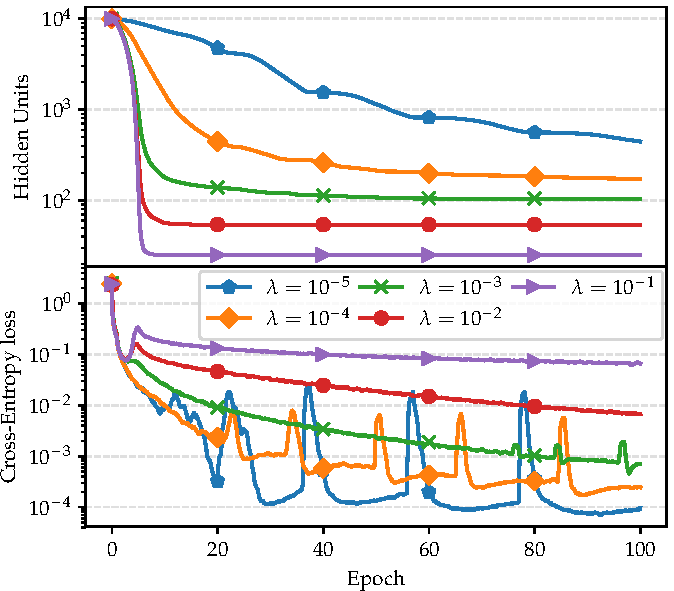
\includegraphics[width=0.5\textwidth]{convergence}
\caption{Evolution of the number of hidden units and loss over time on the \texttt{MNIST} dataset for different $\lambda$ values \label{convergence_plot}}
\end{center}
\end{figure}

\begin{figure}
\begin{center}
  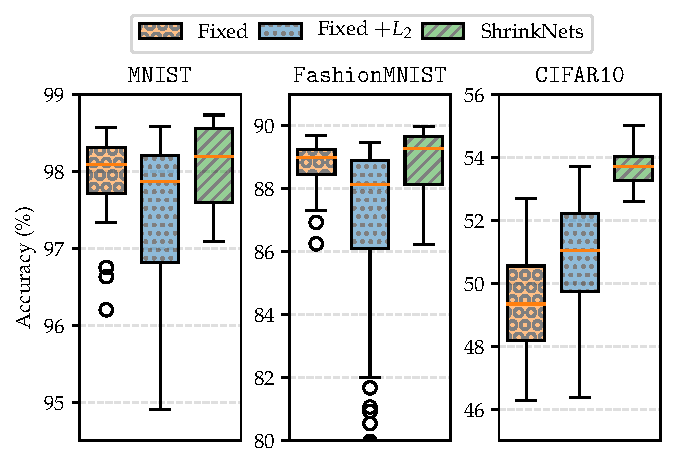
\includegraphics[width=0.5\textwidth]{hyper_opt}
\caption{Distributions of the testing accuracy for different training methods, datasets and architectures using random search\label{hyper_opt_res}}
\end{center}
\end{figure}

\subsection{Comparison between Shrinking and classic Networks}

To demonstrate the value of ShrinkNets in the context of hyper-parameter optimization we set up the following experiment: We consider a \textit{LeNet-5} architecture and assume we do not know the number of channels and neurons. We try to find the best architecture by performing random search on the parameters that define the size. For classic neural networks these parameters are the number of channels for the first two layers and the number of hidden units of the linear layer. For ShrinkNets there is only one parameter $\lambda$. We sampled 50 models of each and trained them, picked the best epoch using the validation accuracy and measured their accuracy on the testing set. Since ShrinkNets can be considered to be regularized in some sense, to make the comparison fair we also considered static networks with an $L2$ regularization factor (also drawn randomly). We summarized the accuracy we obtained on \autoref{hyper_opt_res}. [Should we explain the results]

\section{Future work}

\par Even though the firsts results this techique yields seem promising, there are many area that we could explore to improve it. In the current implementation we only "learn" the number of features (neurons or channels). We could try to augment it with dynamic number of layers as seen in [ref] to be able to determine the entire architecture.
\par We saw on Figure \ref{convergence_plot} that the loss temporarly suffers from the removal of neurons. It is likely that the loss would be more stable if the number of neurons converged faster or neurons disapeared more progressively. This is why we think we should explore proximal gradient methods to optimize the filter vectors and/or randomize neuron removals.
\par During our evaluation we picked small datasets mainly to be able to train many models and have statistically significant distributions. With more computation resources and time, we could see if it generalises to bigger datasets and other architectures like \texttt{ResNet} [ref] (small modifications to the existing code base are required to support them)

\section{Conclusion}
Do the conclusion at the end

\bibliographystyle{ACM-Reference-Format}
\bibliography{sample-bibliography}

\end{document}
